\documentclass{beamer}
\usetheme{ttuStatsCamp}
\usefonttheme{serif}
\usepackage[T1]{fontenc}
\usepackage[utf8]{inputenc}
\usepackage{url}
\usepackage{graphicx}
\usepackage{setspace}
\usepackage[natbibapa]{apacite}
\usepackage{color}
\usepackage{amsmath}
\usepackage{amsfonts}
\usepackage{Sweavel}
\usepackage{listings}

\def\Sweavesize{\scriptsize}
\def\Rcolor{\color{black}}
%\def\Routcolor{\color{red}}
\def\Rcommentcolor{\color{violet}}
\def\Rbackground{\color[gray]{0.85}}
\def\Routbackground{\color[gray]{0.85}}

\lstset{tabsize=2, breaklines=true, style=Rstyle}



\newcommand{\red}[0]{\textcolor{red}}
\newcommand{\green}[0]{\textcolor{green}}
\newcommand{\blue}[0]{\textcolor{blue}}
\newcommand{\comment}[1]{}
\newcommand{\va}[0]{\vspace{12pt}}
\newcommand{\vb}[0]{\vspace{6pt}}
\newcommand{\vc}[0]{\vspace{3pt}}
\newcommand{\vx}[1]{\vspace{#1pt}}

\title[Lecture 5]{Lecture 5: A Bit Advanced Mediation}

\author{Kyle M. Lang}

\institute[TTU IMMAP]{
  Institute for Measurement, Methodology, Analysis \& Policy\\
  Texas Tech University\\
  Lubbock, TX
}

\date{2016 Stats Camp}

\setbeamertemplate{frametitle continuation}{}

\begin{document}

\setkeys{Gin}{width=\textwidth}

\input{sweaveFiles/-001}


\begin{frame}[plain]
  
  \titlepage
  
\end{frame}


\begin{frame}{Outline}
  
  \begin{itemize}
  \item Show how to test for indirect effects in latent variable models
    \va
  \item Discuss the interpretation of indirect effects
    \va
  \item Discuss effect size measures for indirect effects
  \end{itemize}
  
\end{frame}


\begin{frame}{Boring Model}

  So far, all of our models have been similar to:
  \begin{figure}
    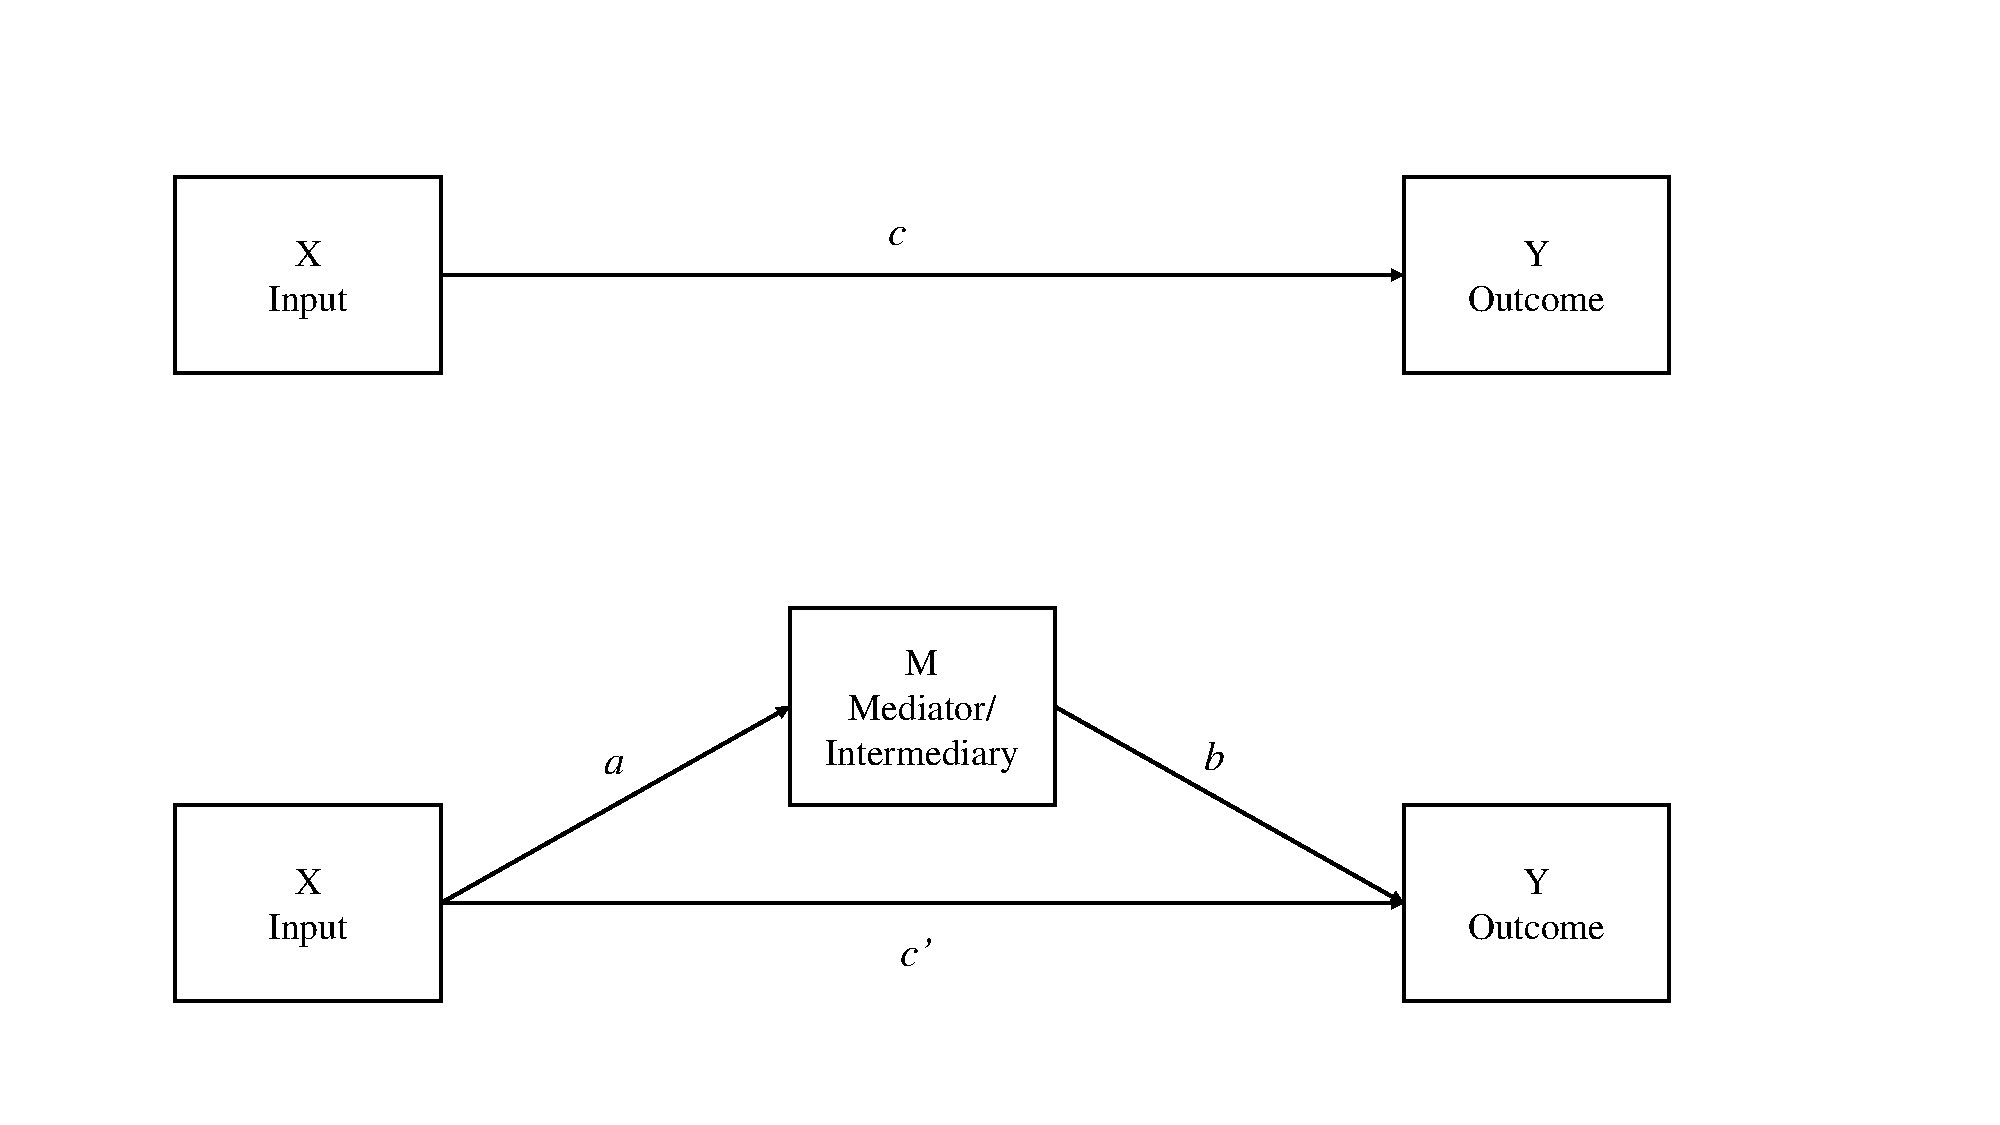
\includegraphics[width=.8\textwidth]{figures/simpleMediationPathDiagram.pdf}
  \end{figure}
  But there is no reason that we need to restrict ourselves to mucking
  about with observed variables.

\end{frame}



\begin{frame}{Better Model}

  We can (and should) test for indirect effects using \emph{latent
    variable models} such as:
  \begin{figure}
    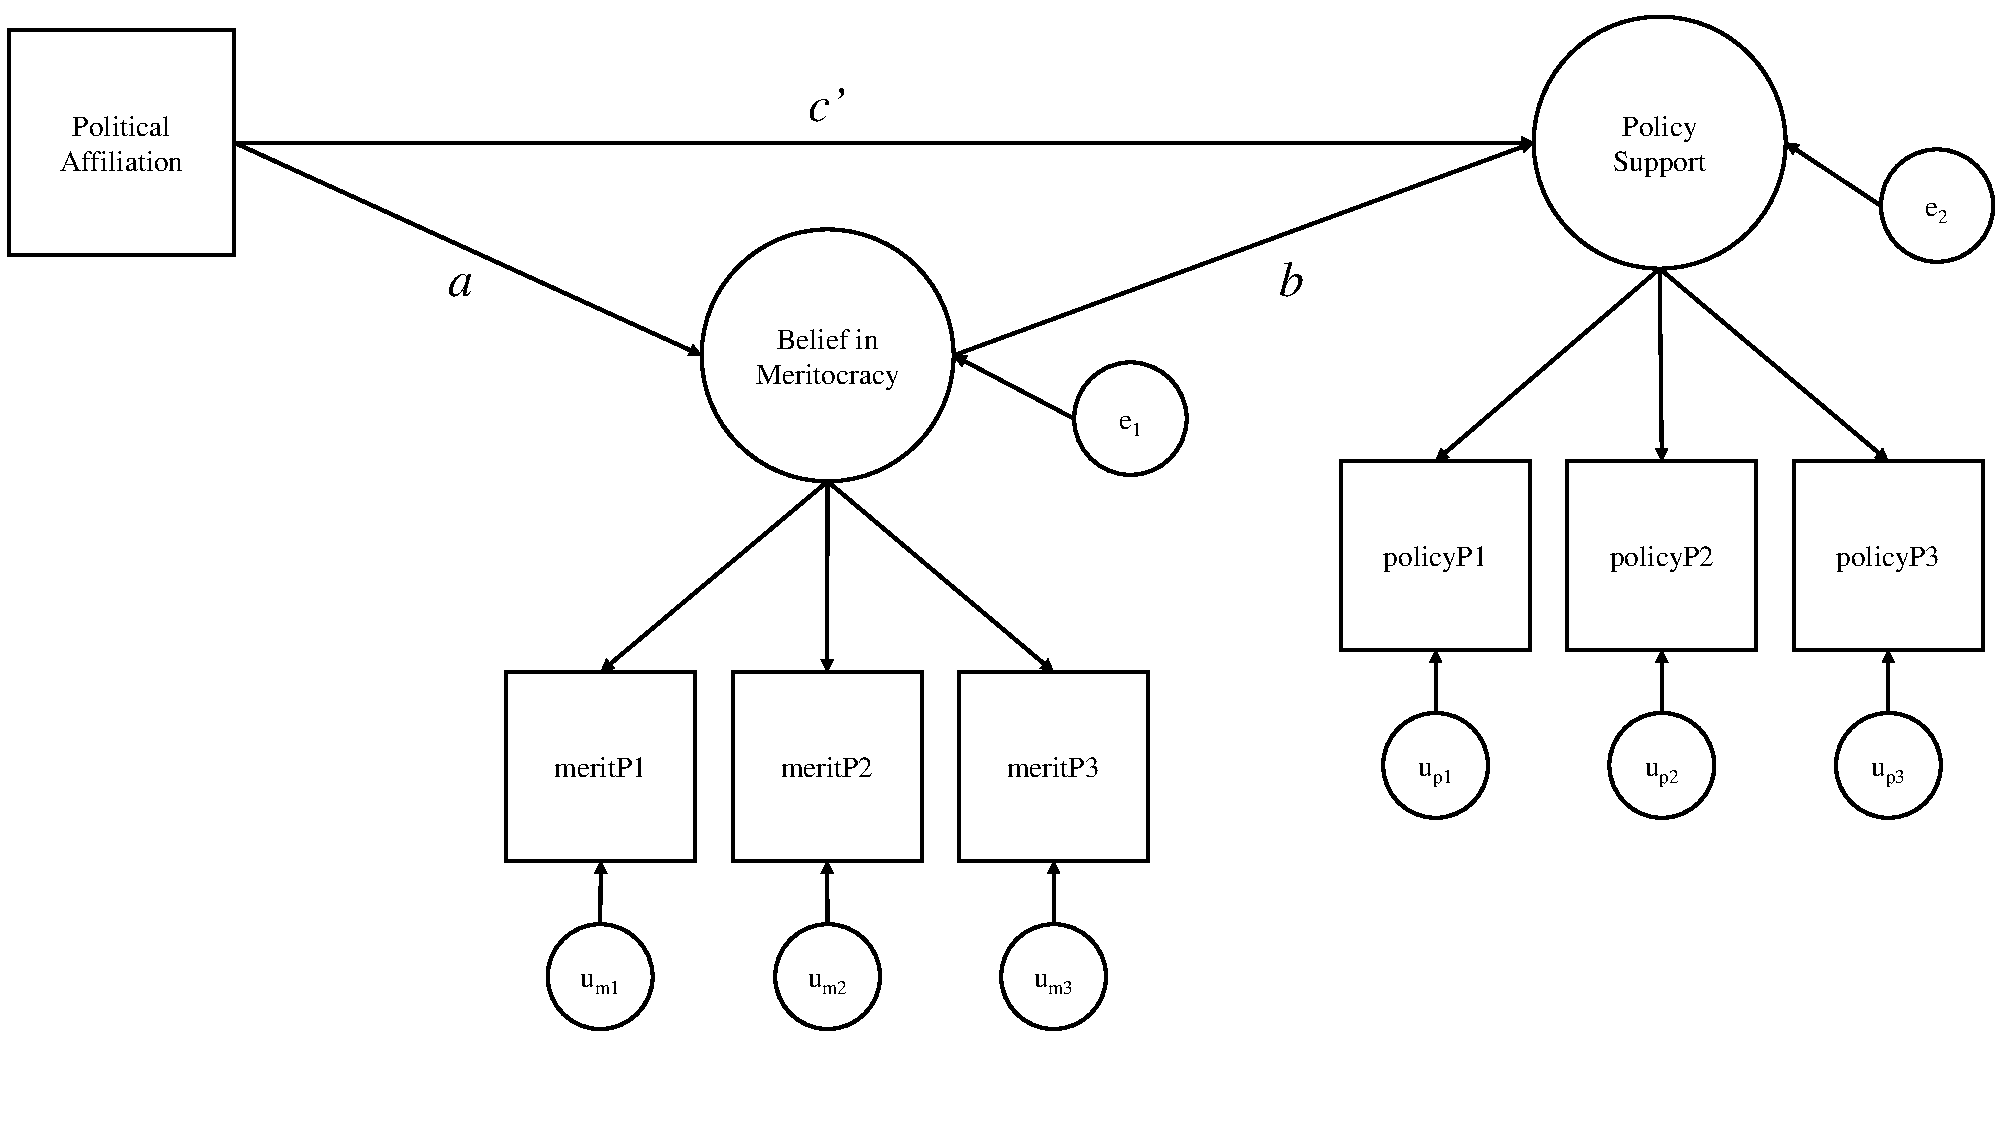
\includegraphics[width=.8\textwidth]{figures/semMedDiagram.pdf}
  \end{figure}
  Measurement error can be a big problem for mediation analysis, so
  latent variable modeling is highly recommended.

\end{frame}



\begin{frame}[allowframebreaks]{Example}
  
\begin{Schunk}
\begin{Sinput}
 library(lavaan)
 dataDir <- "../data/"
 dat1 <- readRDS(paste0(dataDir, "adamsKlpsData.rds"))
 ## Specify the CFA model:
 mod1.1 <- "
 merit =~ meritP1 + meritP2 + meritP3
 policy =~ policyP1 + policyP2 + policyP3
 "
 ## Fit the CFA and check model:
 out1.1 <- cfa(mod1.1, data = dat1, std.lv = TRUE)
 ## Check model fit:
 round(fitMeasures(out1.1)[c("chisq", "df", "pvalue", "cfi", 
                             "tli", "rmsea", "srmr")], 4)
\end{Sinput}
\begin{Soutput}
  chisq      df  pvalue     cfi     tli   rmsea    srmr 
16.8695  8.0000  0.0315  0.9215  0.8529  0.1129  0.0653 
\end{Soutput}
\begin{Sinput}
 summary(out1.1)
\end{Sinput}
\begin{Soutput}
lavaan (0.5-20) converged normally after  22 iterations

  Number of observations                            87

  Estimator                                         ML
  Minimum Function Test Statistic               16.869
  Degrees of freedom                                 8
  P-value (Chi-square)                           0.031

Parameter Estimates:

  Information                                 Expected
  Standard Errors                             Standard

Latent Variables:
                   Estimate  Std.Err  Z-value  P(>|z|)
  merit =~                                            
    meritP1           0.690    0.134    5.155    0.000
    meritP2           0.968    0.142    6.830    0.000
    meritP3           0.748    0.137    5.458    0.000
  policy =~                                           
    policyP1          0.851    0.186    4.570    0.000
    policyP2          0.996    0.167    5.967    0.000
    policyP3          1.121    0.177    6.339    0.000

Covariances:
                   Estimate  Std.Err  Z-value  P(>|z|)
  merit ~~                                            
    policy           -0.336    0.131   -2.563    0.010

Variances:
                   Estimate  Std.Err  Z-value  P(>|z|)
    meritP1           0.865    0.165    5.248    0.000
    meritP2           0.445    0.201    2.211    0.027
    meritP3           0.833    0.172    4.857    0.000
    policyP1          1.836    0.324    5.671    0.000
    policyP2          0.942    0.256    3.683    0.000
    policyP3          0.857    0.297    2.882    0.004
    merit             1.000                           
    policy            1.000                           
\end{Soutput}
\end{Schunk}


\pagebreak

\begin{Schunk}
\begin{Sinput}
 round(fitMeasures(out1)[c("chisq", "df", "pvalue", "cfi", 
                           "tli", "rmsea", "srmr")], 3)
\end{Sinput}
\begin{Soutput}
 chisq     df pvalue    cfi    tli  rmsea   srmr 
41.021 24.000  0.017  0.987  0.981  0.038  0.026 
\end{Soutput}
\end{Schunk}


\end{frame}



\begin{frame}{Interpretation of Indirect Effects}
  
  Although indirect effects are composed parameters, they have direct
  interpretations, independent of the interpretations of their
  constituent paths:
  \vb
  \begin{itemize}
  \item The $X \rightarrow M \rightarrow Y$ indirect effect $ab$ is
    interpreted as:
    \vb
    \begin{itemize}
    \item The expected change in $Y$ for a unit change in $X$ that
      is transmitted indirectly through $M$, or...
      \vb
    \item For a unit change in $X$, $Y$ is expected to change by
      $ab$ units, indirectly through $M$, or...
      \vb
    \item Participants who differ by one unit on $X$ are expect
      to differ by $ab$ units on $Y$ as a results of the effect
      of $X$ on $M$ which, in turn, affects $Y$.
    \end{itemize}
    \va
  \item The interpretation/scaling of the indirect effect is entirely
    defined by the input $X$ and outcome $Y$
    \vb
    \begin{itemize}
    \item The scaling of the intermediary variable $M$ does not affect
      the interpretation of the indirect effect.
    \end{itemize}
  \end{itemize}
  
\end{frame}
  
  
\begin{frame}{Partially Standardized Indirect Effect}
  
  \begin{align*}
    ab_{ps} &= \frac{ab}{SD_Y}\\
    c'_{ps} &= \frac{c'}{SD_Y}\\
    c_{ps} &= \frac{c}{SD_Y} = ab_{ps} + c'_{ps}
  \end{align*}
  
  \begin{itemize}
    \item Simple
    \item Removes binding to the scale of $Y$
    \item Still scale-bound by $X$
    \item Not clear what constitutes a ``large'' effect
  \end{itemize}
  
\end{frame}



\begin{frame}{Completely Standardized Indirect Effect}
  
  \begin{align*}
    ab_{cs} &= \frac{SD_X ab}{SD_Y}\\
    c'_{cs} &= \frac{SD_X c'}{SD_Y}\\
    c_{cs} &= \frac{SD_X c}{SD_Y} = ab_{cs} + c'_{cs}
  \end{align*}
  
  \begin{itemize}
    \item Simple
    \item Removes all scale binding
    \item Not clear what constitutes a ``large'' effect
  \end{itemize}
  
\end{frame}


\begin{frame}{Ratio of the Indirect Effect to the Total Effect}
  
  \begin{align*}
    P_M = \frac{ab}{c} = \frac{ab}{c' + ab}
  \end{align*}
  
  \begin{itemize}
  \item Very simple
  \item Not bounded by 0 and 1
  \item Explodes toward $\pm \infty$ as $c\rightarrow 0$
  \item Very unstable
    \begin{itemize}
    \item High between-sample variability
    \item Requires $N \geq 500$
    \end{itemize}
  \end{itemize}
\end{frame}



\begin{frame}{Ratio of the Indirect Effect to the Direct Effect}
  
  \begin{align*}
    R_M = \frac{ab}{c'} = \frac{P_M}{1 - P_M}
  \end{align*}
  
  \begin{itemize}
  \item Very simple
  \item Not bounded by 0 and 1
  \item Explodes toward $\pm \infty$ as $c'\rightarrow 0$
  \item Very unstable
    \begin{itemize}
    \item High between-sample variability
    \item Requires $N \geq 2000$
    \end{itemize}
  \end{itemize}
  
\end{frame}


\begin{frame}{Proportion of Variance in $Y$ Explained by the Indirect Effect}
  
  Developed by \citet{fairchildEtAl:2009}.
  \begin{itemize}
    \item Given a non-zero total effect, represents the proportion of
      variance in Y accounted for by the indirect effect.
  \end{itemize}
  
  \begin{align*}
    R_{med}^2 = r_{MY}^2 - \left( R_{Y.MX}^2-r_{XY}^2 \right)
  \end{align*}

  \begin{itemize}
  \item Mostly sensible interpretation
  \item Predicated on the assumption that $\beta_{YX} \neq 0$
  \item $|ab| > |c| \Rightarrow R_{med}^2 < 0$
    \begin{itemize}
    \item Not a strict proportion
    \end{itemize}
  \end{itemize}
  
\end{frame}


\begin{frame}{Kappa Squared}
  
  Developed by \citet{preacherKelley:2011}.
  \begin{itemize}
  \item Gives the proportion of the \emph{maximum possible} indirect
    effect represented by $ab$.
  \end{itemize}
  
  \begin{align*}
    \kappa^2 = \frac{ab}{\text{max}(ab)}
  \end{align*}
  
  \begin{itemize}
  \item Bounded by 0 and 1
  \item Values closer to 1.0 indicate a bigger effect
  \item A bit of a pain to calculate.
  \end{itemize}
  
\end{frame}


\begin{frame}{Computing $\text{max}(ab)$}
  
  \begin{align*}
    a &\in \left\{ 
    \frac{
      \sigma_{YM} \sigma_{YX} \pm 
      \sqrt{ \sigma_M^2 \sigma_Y^2 - \sigma_{YM}^2 }
      \sqrt{ \sigma_X^2 \sigma_Y^2 - \sigma_{YX}^2 } 
    }{ 
      \sigma_X^2 \sigma_Y^2 
    }
    \right\} 
    = [a_{low}, a_{high}],
    \\
    \\
    b &\in \left\{
    \pm \frac{
      \sqrt{ \sigma_X^2 \sigma_Y^2 - \sigma_{YX}^2 }
    }{
      \sqrt{ \sigma_X^2 \sigma_M^2 - \sigma_{MX}^2 }
    }
    \right\} = [b_{low}, b_{high}],
  \end{align*}
  
  \begin{align*}
    \text{max}(a) = \left\{ \begin{array}{lll}
      a_{high}, & \text{ if } & \hat{a} > 0\\
      a_{low}, & \text{ if } & \hat{a} < 0
    \end{array}
    \right.,~~
    \text{max}(b) = \left\{ \begin{array}{lll}
      b_{high}, & \text{ if } & \hat{b} > 0\\
      b_{low}, & \text{ if } & \hat{b} < 0
    \end{array}
    \right.,
  \end{align*}
  
  \begin{align*}
    \text{max}(ab) = \text{max}(a) \text{max}(b)
  \end{align*}
  
\end{frame}


\begin{frame}[allowframebreaks]{Example}
    
\begin{Schunk}
\begin{Sinput}
 mod3 <- "
 att3 ~ att2 + b2*conf2 + cp2*horn2
 att2 ~ att1 + b1*conf1 + cp1*horn1
 
 conf3 ~ conf2 + a2*horn2
 conf2 ~ conf1 + a1*horn1
 
 horn3 ~ horn2
 horn2 ~ horn1
 
 horn3 ~~ conf3 + att3
 conf3 ~~ att3
 
 horn2 ~~ conf2 + att2
 conf2 ~~ att2
 
 a1 == a2
 b1 == b2
 cp1 == cp2
 "
 out3 <- sem(mod3, data = dat1)
 summary(out3)
\end{Sinput}
\begin{Soutput}
lavaan (0.5-20) converged normally after  46 iterations

  Number of observations                           500

  Estimator                                         ML
  Minimum Function Test Statistic              294.220
  Degrees of freedom                                18
  P-value (Chi-square)                           0.000

Parameter Estimates:

  Information                                 Expected
  Standard Errors                             Standard

Regressions:
                   Estimate  Std.Err  Z-value  P(>|z|)
  att3 ~                                              
    att2              0.497    0.035   14.234    0.000
    conf2     (b2)    0.098    0.019    5.200    0.000
    horn2    (cp2)    0.083    0.072    1.157    0.247
  att2 ~                                              
    att1              0.530    0.040   13.345    0.000
    conf1     (b1)    0.098    0.019    5.200    0.000
    horn1    (cp1)    0.083    0.072    1.157    0.247
  conf3 ~                                             
    conf2             0.684    0.035   19.602    0.000
    horn2     (a2)    0.493    0.107    4.596    0.000
  conf2 ~                                             
    conf1             0.623    0.032   19.546    0.000
    horn1     (a1)    0.493    0.107    4.596    0.000
  horn3 ~                                             
    horn2             0.826    0.030   27.609    0.000
  horn2 ~                                             
    horn1             0.714    0.024   29.181    0.000

Covariances:
                   Estimate  Std.Err  Z-value  P(>|z|)
  conf3 ~~                                            
    horn3             1.016    0.155    6.556    0.000
  att3 ~~                                             
    horn3             0.322    0.093    3.483    0.000
    conf3             3.574    0.465    7.691    0.000
  conf2 ~~                                            
    horn2             0.836    0.124    6.721    0.000
  att2 ~~                                             
    horn2             0.273    0.083    3.289    0.001
    conf2             2.027    0.400    5.067    0.000

Variances:
                   Estimate  Std.Err  Z-value  P(>|z|)
    att3              6.019    0.381   15.811    0.000
    att2              6.041    0.382   15.811    0.000
    conf3            15.814    1.000   15.811    0.000
    conf2            12.570    0.795   15.811    0.000
    horn3             0.695    0.044   15.811    0.000
    horn2             0.560    0.035   15.811    0.000

Constraints:
                                               |Slack|
    a1 - (a2)                                    0.000
    b1 - (b2)                                    0.000
    cp1 - (cp2)                                  0.000
\end{Soutput}
\begin{Sinput}
 chiDiff <- fitMeasures(out3)["chisq"] -
     fitMeasures(out1)["chisq"]
 dfDiff <- fitMeasures(out3)["df"] -
     fitMeasures(out1)["df"]
 pchisq(chiDiff, dfDiff, lower = FALSE)
\end{Sinput}
\begin{Soutput}
     chisq 
0.02684148 
\end{Soutput}
\end{Schunk}


\pagebreak

\begin{Schunk}
\begin{Sinput}
 mod4 <- "
 att3 ~ att2 + b2*conf2 + cp*horn1
 att2 ~ att1 + b1*conf1
 
 conf3 ~ conf2 + a2*horn2
 conf2 ~ conf1 + a1*horn1
 
 att2 + att3 ~ income
 conf2 + conf3 ~ income 
 horn2 + horn3 ~ income
 
 horn3 ~ horn2
 horn2 ~ horn1
 
 horn3 ~~ conf3 + att3
 conf3 ~~ att3
 
 horn2 ~~ conf2 + att2
 conf2 ~~ att2
 
 ab := a1*b2
 "
 out4 <- sem(mod4, data = dat1, se = "boot", boot = nBoot)
 summary(out4)
\end{Sinput}
\begin{Soutput}
lavaan (0.5-20) converged normally after  63 iterations

  Number of observations                           500

  Estimator                                         ML
  Minimum Function Test Statistic              219.789
  Degrees of freedom                                16
  P-value (Chi-square)                           0.000

Parameter Estimates:

  Information                                 Observed
  Standard Errors                            Bootstrap
  Number of requested bootstrap draws             2000
  Number of successful bootstrap draws            2000

Regressions:
                   Estimate  Std.Err  Z-value  P(>|z|)
  att3 ~                                              
    att2              0.513    0.039   13.099    0.000
    conf2     (b2)    0.022    0.027    0.826    0.409
    horn1     (cp)   -0.119    0.084   -1.418    0.156
  att2 ~                                              
    att1              0.477    0.043   10.980    0.000
    conf1     (b1)    0.084    0.028    3.048    0.002
  conf3 ~                                             
    conf2             0.488    0.041   11.803    0.000
    horn2     (a2)    0.492    0.160    3.076    0.002
  conf2 ~                                             
    conf1             0.543    0.037   14.594    0.000
    horn1     (a1)    0.175    0.146    1.204    0.228
  att2 ~                                              
    income            0.052    0.013    4.108    0.000
  att3 ~                                              
    income            0.057    0.012    4.853    0.000
  conf2 ~                                             
    income            0.110    0.016    6.871    0.000
  conf3 ~                                             
    income            0.148    0.018    8.206    0.000
  horn2 ~                                             
    income            0.016    0.003    5.698    0.000
  horn3 ~                                             
    income            0.013    0.004    3.555    0.000
    horn2             0.780    0.033   23.921    0.000
  horn2 ~                                             
    horn1             0.654    0.026   25.525    0.000

Covariances:
                   Estimate  Std.Err  Z-value  P(>|z|)
  conf3 ~~                                            
    horn3             0.915    0.152    6.020    0.000
  att3 ~~                                             
    horn3             0.322    0.092    3.489    0.000
    conf3             2.971    0.412    7.215    0.000
  conf2 ~~                                            
    horn2             0.678    0.112    6.026    0.000
  att2 ~~                                             
    horn2             0.203    0.083    2.428    0.015
    conf2             1.601    0.382    4.194    0.000

Variances:
                   Estimate  Std.Err  Z-value  P(>|z|)
    att3              5.771    0.351   16.431    0.000
    att2              5.821    0.362   16.099    0.000
    conf3            14.066    0.828   16.988    0.000
    conf2            11.512    0.729   15.792    0.000
    horn2             0.529    0.033   16.004    0.000
    horn3             0.677    0.040   16.788    0.000

Defined Parameters:
                   Estimate  Std.Err  Z-value  P(>|z|)
    ab                0.004    0.007    0.559    0.576
\end{Soutput}
\begin{Sinput}
 parameterEstimates(out4, boot = "bca.simple")[ , -c(1 : 3)]
\end{Sinput}
\begin{Soutput}
   label     est    se      z pvalue ci.lower ci.upper
1          0.513 0.039 13.099  0.000    0.438    0.589
2     b2   0.022 0.027  0.826  0.409   -0.030    0.076
3     cp  -0.119 0.084 -1.418  0.156   -0.275    0.051
4          0.477 0.043 10.980  0.000    0.396    0.565
5     b1   0.084 0.028  3.048  0.002    0.029    0.139
6          0.488 0.041 11.803  0.000    0.410    0.569
7     a2   0.492 0.160  3.076  0.002    0.186    0.818
8          0.543 0.037 14.594  0.000    0.464    0.614
9     a1   0.175 0.146  1.204  0.228   -0.099    0.468
10         0.052 0.013  4.108  0.000    0.028    0.077
11         0.057 0.012  4.853  0.000    0.033    0.079
12         0.110 0.016  6.871  0.000    0.079    0.141
13         0.148 0.018  8.206  0.000    0.114    0.183
14         0.016 0.003  5.698  0.000    0.011    0.022
15         0.013 0.004  3.555  0.000    0.005    0.019
16         0.780 0.033 23.921  0.000    0.714    0.844
17         0.654 0.026 25.525  0.000    0.601    0.703
18         0.915 0.152  6.020  0.000    0.633    1.225
19         0.322 0.092  3.489  0.000    0.143    0.508
20         2.971 0.412  7.215  0.000    2.207    3.834
21         0.678 0.112  6.026  0.000    0.466    0.903
22         0.203 0.083  2.428  0.015    0.040    0.369
23         1.601 0.382  4.194  0.000    0.870    2.387
24         5.771 0.351 16.431  0.000    5.130    6.509
25         5.821 0.362 16.099  0.000    5.171    6.590
26        14.066 0.828 16.988  0.000   12.623   15.934
27        11.512 0.729 15.792  0.000   10.207   13.077
28         0.529 0.033 16.004  0.000    0.472    0.602
29         0.677 0.040 16.788  0.000    0.606    0.765
30         1.809 0.000     NA     NA    1.809    1.809
31         1.470 0.000     NA     NA    1.470    1.470
32         3.939 0.000     NA     NA    3.939    3.939
33         5.753 0.000     NA     NA    5.753    5.753
34         8.748 0.000     NA     NA    8.748    8.748
35         8.475 0.000     NA     NA    8.475    8.475
36        16.763 0.000     NA     NA   16.763   16.763
37        28.025 0.000     NA     NA   28.025   28.025
38        39.156 0.000     NA     NA   39.156   39.156
39       136.353 0.000     NA     NA  136.353  136.353
40    ab   0.004 0.007  0.559  0.576   -0.003    0.031
\end{Soutput}
\end{Schunk}


\pagebreak

\begin{Schunk}
\begin{Sinput}
 ## Completely Standardized:
 abCS <- (sdX * ab) / sdY
 abCS
\end{Sinput}
\begin{Soutput}
[1] 0.1345859
\end{Soutput}
\begin{Sinput}
 cPrimeCS <- (sdX * cPrime) / sdY
 cPrimeCS
\end{Sinput}
\begin{Soutput}
       cp 
0.1790413 
\end{Soutput}
\begin{Sinput}
 cCS <- abCS + cPrimeCS
 cCS
\end{Sinput}
\begin{Soutput}
       cp 
0.3136272 
\end{Soutput}
\end{Schunk}


\pagebreak

\begin{Schunk}
\begin{Sinput}
 mod3 <- "
 fX =~ x1 + x2 + x3
 fZ =~ z1 + z2 + z3
 fY =~ y1 + y2 + y3
 fXZ =~ x1z1R + x1z2R + x1z3R +
 x2z1R + x2z2R + x2z3R +
 x3z1R + x3z2R + x3z3R
 
 fY ~ fX + fZ + fXZ
 
 fX ~~ fZ
 fX ~~ 0*fXZ
 fZ ~~ 0*fXZ
 
 x1z1R ~~ x1z2R + x1z3R + x2z1R + x3z1R
 x1z2R ~~ x1z3R + x2z2R + x3z2R
 x1z3R ~~ x2z3R + x3z3R
 
 x2z1R ~~ x2z2R + x2z3R + x3z1R
 x2z2R ~~ x2z3R + x3z2R
 x2z3R ~~ x3z3R
 
 x3z1R ~~ x3z2R + x3z3R
 x3z2R ~~ x3z3R
 "
 out3 <- sem(mod3, data = dat2, std.lv = TRUE)
 summary(out3)
\end{Sinput}
\begin{Soutput}
lavaan (0.5-20) converged normally after  53 iterations

  Number of observations                           500

  Estimator                                         ML
  Minimum Function Test Statistic               74.899
  Degrees of freedom                               113
  P-value (Chi-square)                           0.998

Parameter Estimates:

  Information                                 Expected
  Standard Errors                             Standard

Latent Variables:
                   Estimate  Std.Err  Z-value  P(>|z|)
  fX =~                                               
    x1                0.670    0.043   15.424    0.000
    x2                0.660    0.043   15.256    0.000
    x3                0.704    0.045   15.569    0.000
  fZ =~                                               
    z1                0.738    0.048   15.342    0.000
    z2                0.734    0.048   15.156    0.000
    z3                0.718    0.046   15.602    0.000
  fY =~                                               
    y1                0.396    0.046    8.545    0.000
    y2                0.369    0.044    8.441    0.000
    y3                0.383    0.045    8.558    0.000
  fXZ =~                                              
    x1z1R             0.361    0.053    6.833    0.000
    x1z2R             0.427    0.056    7.615    0.000
    x1z3R             0.432    0.053    8.190    0.000
    x2z1R             0.558    0.056    9.914    0.000
    x2z2R             0.616    0.062   10.008    0.000
    x2z3R             0.520    0.057    9.153    0.000
    x3z1R             0.516    0.059    8.805    0.000
    x3z2R             0.626    0.063   10.007    0.000
    x3z3R             0.521    0.058    8.936    0.000

Regressions:
                   Estimate  Std.Err  Z-value  P(>|z|)
  fY ~                                                
    fX                1.658    0.239    6.930    0.000
    fZ               -0.074    0.099   -0.750    0.453
    fXZ               0.488    0.120    4.049    0.000

Covariances:
                   Estimate  Std.Err  Z-value  P(>|z|)
  fX ~~                                               
    fZ                0.232    0.058    3.987    0.000
    fXZ               0.000                           
  fZ ~~                                               
    fXZ               0.000                           
  x1z1R ~~                                            
    x1z2R             0.273    0.032    8.397    0.000
    x1z3R             0.309    0.033    9.358    0.000
    x2z1R             0.232    0.031    7.566    0.000
    x3z1R             0.235    0.032    7.376    0.000
  x1z2R ~~                                            
    x1z3R             0.231    0.032    7.243    0.000
    x2z2R             0.211    0.035    5.982    0.000
    x3z2R             0.250    0.041    6.163    0.000
  x1z3R ~~                                            
    x2z3R             0.213    0.030    7.010    0.000
    x3z3R             0.213    0.034    6.312    0.000
  x2z1R ~~                                            
    x2z2R             0.247    0.043    5.787    0.000
    x2z3R             0.252    0.040    6.368    0.000
    x3z1R             0.233    0.033    7.103    0.000
  x2z2R ~~                                            
    x2z3R             0.304    0.043    7.086    0.000
    x3z2R             0.199    0.040    5.018    0.000
  x2z3R ~~                                            
    x3z3R             0.139    0.030    4.570    0.000
  x3z1R ~~                                            
    x3z2R             0.212    0.041    5.116    0.000
    x3z3R             0.260    0.040    6.454    0.000
  x3z2R ~~                                            
    x3z3R             0.157    0.041    3.846    0.000

Variances:
                   Estimate  Std.Err  Z-value  P(>|z|)
    x1                0.511    0.042   12.093    0.000
    x2                0.514    0.042   12.221    0.000
    x3                0.548    0.046   11.977    0.000
    z1                0.523    0.052   10.142    0.000
    z2                0.546    0.052   10.444    0.000
    z3                0.461    0.048    9.704    0.000
    y1                0.495    0.043   11.398    0.000
    y2                0.542    0.044   12.334    0.000
    y3                0.444    0.040   11.179    0.000
    x1z1R             0.743    0.050   14.912    0.000
    x1z2R             0.754    0.055   13.682    0.000
    x1z3R             0.694    0.050   13.824    0.000
    x2z1R             0.641    0.057   11.332    0.000
    x2z2R             0.708    0.067   10.575    0.000
    x2z3R             0.671    0.056   12.009    0.000
    x3z1R             0.736    0.060   12.310    0.000
    x3z2R             0.724    0.070   10.277    0.000
    x3z3R             0.707    0.060   11.823    0.000
    fX                1.000                           
    fZ                1.000                           
    fY                1.000                           
    fXZ               1.000                           
\end{Soutput}
\end{Schunk}


\end{frame}


\begin{frame}[allowframebreaks]{Compute $\kappa^2$}

\begin{Schunk}
\begin{Sinput}
 parameterEstimates(out2.1, boot = bootType)[ , -c(1 : 3)]
\end{Sinput}
\begin{Soutput}
     label    est    se      z pvalue ci.lower ci.upper
1       b1 -0.008 0.145 -0.052  0.959   -0.286    0.275
2       b2  0.595 0.142  4.184  0.000    0.317    0.861
3       cp  0.134 0.076  1.763  0.078   -0.019    0.281
4      d21 -0.301 0.110 -2.733  0.006   -0.508   -0.076
5       a2  0.090 0.072  1.253  0.210   -0.073    0.220
6       a1 -0.266 0.061 -4.384  0.000   -0.384   -0.148
7           0.987 0.164  6.013  0.000    0.733    1.390
8           0.689 0.094  7.309  0.000    0.537    0.919
9           0.719 0.112  6.389  0.000    0.535    0.980
10          2.444 0.000     NA     NA    2.444    2.444
11     ab1  0.002 0.040  0.050  0.960   -0.080    0.081
12     ab2  0.053 0.044  1.215  0.225   -0.031    0.146
13  fullIE  0.048 0.026  1.822  0.068    0.012    0.117
14 totalIE  0.103 0.048  2.145  0.032    0.011    0.202
\end{Soutput}
\end{Schunk}


\pagebreak

\begin{Schunk}
\begin{Sinput}
 ## Possible range of a:
 aMarg <- sqrt(s2M * s2Y - sYM^2) * sqrt(s2X * s2Y - sYX^2)
 aInt <- c(
     (sYM * sYX - aMarg) / (s2X * s2Y),
     (sYM * sYX + aMarg) / (s2X * s2Y)
 )
 aInt
\end{Sinput}
\begin{Soutput}
[1] -0.4378558  0.5793099
\end{Soutput}
\begin{Sinput}
 ##
 ## Possible range of b:
 bMarg <- sqrt(s2X * s2Y - sYX^2) / sqrt(s2X * s2M - sMX^2)
 bInt <- c(-1 * bMarg, bMarg)
 bInt
\end{Sinput}
\begin{Soutput}
[1] -1.289996  1.289996
\end{Soutput}
\begin{Sinput}
 ##
 ## max(a):
 aMax <- ifelse(coef(out2)["a"] < 0,
                aInt[1],
                aInt[2])
 aMax
\end{Sinput}
\begin{Soutput}
        a 
0.5793099 
\end{Soutput}
\begin{Sinput}
 ##
 ## max(b)
 bMax <- ifelse(coef(out2)["b"] < 0,
                bInt[1],
                bInt[2])
 bMax
\end{Sinput}
\begin{Soutput}
       b 
1.289996 
\end{Soutput}
\begin{Sinput}
 ##
 ## max(ab)
 abMax <- aMax * bMax
 abMax
\end{Sinput}
\begin{Soutput}
        a 
0.7473075 
\end{Soutput}
\begin{Sinput}
 ##
 ## Kappa Squared:
 k2 <- ab / abMax
 k2
\end{Sinput}
\begin{Soutput}
        a 
0.1359491 
\end{Soutput}
\end{Schunk}


\end{frame}


\begin{frame}{Practice}
  
\begin{Schunk}
\begin{Sinput}
 ## Three-way interaction model:
 out1.3 <- lm(agree ~ open*conc*neuro, data = dat1)
 summary(out1.3)
\end{Sinput}
\begin{Soutput}
Call:
lm(formula = agree ~ open * conc * neuro, data = dat1)

Residuals:
     Min       1Q   Median       3Q      Max 
-2.79789 -0.41779  0.09925  0.47556  2.10928 

Coefficients:
                Estimate Std. Error t value Pr(>|t|)    
(Intercept)     -0.58747    0.96633  -0.608  0.54328    
open             1.27903    0.25747   4.968 7.23e-07 ***
conc             1.20831    0.26559   4.550 5.63e-06 ***
neuro            0.73766    0.32240   2.288  0.02222 *  
open:conc       -0.29722    0.06935  -4.286 1.89e-05 ***
open:neuro      -0.21616    0.08091  -2.672  0.00760 ** 
conc:neuro      -0.25632    0.08244  -3.109  0.00190 ** 
open:conc:neuro  0.06541    0.02028   3.225  0.00128 ** 
---
Signif. codes:  0 ‘***’ 0.001 ‘**’ 0.01 ‘*’ 0.05 ‘.’ 0.1 ‘ ’ 1

Residual standard error: 0.6945 on 2544 degrees of freedom
Multiple R-squared:  0.07189,	Adjusted R-squared:  0.06933 
F-statistic: 28.15 on 7 and 2544 DF,  p-value: < 2.2e-16
\end{Soutput}
\end{Schunk}


Suppose:
\begin{enumerate}
\item $\Sigma$ is given by:
\begin{Schunk}
\begin{Sinput}
 ## Test Differences between Indirect Effects
 ## in Serial Multiple Mediator Model (Method 1):
 mod2.3 <- "
 policy ~ cp*polAffil + b1*merit + b2*sysRac
 merit ~ a1*polAffil
 sysRac ~ a2*polAffil + d21*merit
 
 ab1 := a1*b1
 ab2 := a2*b2
 fullIE := a1*d21*b2
 totalIE := ab1 + ab2 + fullIE 
 
 fullIE == ab1
 fullIE == ab2
 "
 out2.3 <- 
     sem(mod2.3, data = dat1, se = "boot", boot = nBoot)
 summary(out2.3)
\end{Sinput}
\begin{Soutput}
lavaan (0.5-20) converged normally after 213 iterations

  Number of observations                            87

  Estimator                                         ML
  Minimum Function Test Statistic                1.334
  Degrees of freedom                                 2
  P-value (Chi-square)                           0.513

Parameter Estimates:

  Information                                 Observed
  Standard Errors                            Bootstrap
  Number of requested bootstrap draws             2500
  Number of successful bootstrap draws            2500

Regressions:
                   Estimate  Std.Err  Z-value  P(>|z|)
  policy ~                                            
    polAffil  (cp)    0.108    0.084    1.281    0.200
    merit     (b1)   -0.150    0.047   -3.183    0.001
    sysRac    (b2)    0.521    0.125    4.157    0.000
  merit ~                                             
    polAffil  (a1)   -0.271    0.057   -4.750    0.000
  sysRac ~                                            
    polAffil  (a2)    0.078    0.025    3.125    0.002
    merit    (d21)   -0.287    0.075   -3.814    0.000

Variances:
                   Estimate  Std.Err  Z-value  P(>|z|)
    policy            1.001    0.171    5.854    0.000
    merit             0.719    0.114    6.330    0.000
    sysRac            0.690    0.090    7.632    0.000

Defined Parameters:
                   Estimate  Std.Err  Z-value  P(>|z|)
    ab1               0.041    0.014    2.983    0.003
    ab2               0.041    0.014    2.983    0.003
    fullIE            0.041    0.014    2.983    0.003
    totalIE           0.122    0.041    2.983    0.003

Constraints:
                                               |Slack|
    fullIE - (ab1)                               0.000
    fullIE - (ab2)                               0.000
\end{Soutput}
\begin{Sinput}
 ## Conduct a chi-squared difference test:
 chiDiff <- fitMeasures(out2.3)["chisq"] - 
     fitMeasures(out2.1)["chisq"]
 dfDiff <- fitMeasures(out2.3)["df"] - 
     fitMeasures(out2.1)["df"]
 pchisq(chiDiff, dfDiff, lower = FALSE)
\end{Sinput}
\begin{Soutput}
    chisq 
0.5131246 
\end{Soutput}
\end{Schunk}

\va
\item The estimated paths are:
  \begin{itemize}
  \item $a = $ 0.2
    \vb
  \item $b = $ 0.246
    \vb
  \item $ab = $ 0.049
  \end{itemize}
  \end{enumerate}
  \va
  Compute $\kappa^2$ for the estimated $ab$.
  
\end{frame}

\begin{frame}{References}
\bibliographystyle{apacite}
\bibliography{../../bibtexStuff/dissRefsList}
\end{frame}


\end{document}
